% Complete Section 7.2, original PDF 93-95 / printed 83-85.
% block: koszul-complex-heading page:93 type:section
\subsection{{Koszul 复形}}\label{sec:koszul-complex}

% block: koszul-identity-vector-field page:93 type:ordinary-paragraph
{对 $x\in\Omega\subset\mathbb R^n$, 可将切空间 $T_x\Omega$ 与 $\mathbb R^n$ 等同, 因而为每个点 $x\in\Omega$ 指定同一个 $x$, 但将其看作切空间中的向量, 就得到一个向量场. 此恒等向量场见 Figure~\ref{fig:identity-vector-field}.}

% block: koszul-differential-definition page:93 type:ordinary-paragraph
{$k$-形式 $\omega$ 的 \emph{Koszul 微分} $\kappa\omega=\omega\lrcorner\operatorname{id}$, 是将 $\omega$ 与恒等向量场缩并得到的 $(k-1)$-形式. 即}
\[
\begin{gathered}
(\kappa\omega)_x(v_1,\ldots,v_{k-1})=\omega_x(x,v_1,\ldots,v_{k-1}),\\
x\in\Omega,\ v_1,\ldots,v_{k-1}\in\mathbb R^n,
\end{gathered}
\]
{其中右端括号内的点 $x$ 被看作切向量. 在 $0$-形式上, 规定 $\kappa$ 为零. 由于 $\omega(x,x,\ldots)\equiv0$, 有 $\kappa\circ\kappa=0$, 所以 $\kappa$ 确实是微分. 注意}
\[
\kappa(dx^i)=x^i,
\]
{即基本 $1$-形式 $dx^i$ 的 Koszul 微分是第 $i$ 个坐标函数. 由于 $\kappa$ 通过与向量场缩并来定义, 它满足 Leibniz 法则:}
\[
\kappa(\omega\wedge\mu)=(\kappa\omega)\wedge\mu+(-1)^k\omega\wedge(\kappa\mu).
\]
{特别地, 对任意微分形式 $\omega$ 和任意函数 $f$, 有 $\kappa(f\omega)=f\kappa\omega$, 因而例如 $\kappa(f\,dx^i)=f\,x^i$. 这些法则完全确定了 $\kappa$. 例如,}
\[
\begin{aligned}
\kappa(dx^i\wedge dx^j)&=x^i\,dx^j-x^j\,dx^i,\\
\kappa(dx^i\wedge dx^j\wedge dx^k)&=x^i\,dx^j\wedge dx^k-x^j\,dx^i\wedge dx^k+x^k\,dx^i\wedge dx^j.
\end{aligned}
\]

% block: identity-vector-field-figure page:94 type:figure
\begin{figure}[htbp]\centering
\includegraphics[page=94,trim=150bp 430bp 118bp 62bp,clip,width=.54\linewidth]{../input/source/Finite Element Exterior Calculus.pdf}
\caption{{恒等向量场.}}\label{fig:identity-vector-field}
\end{figure}

% block: koszul-vector-proxies page:94 type:ordinary-paragraph
{若将 $1$-形式与向量场等同, 则 $\kappa$ 对应于向量场与 $x$ 的点积 (更准确地说, 是与恒等向量场的点积). 应用于三维中的 $2$-形式时, $\kappa$ 是与 $x$ 的叉积; 在 $3$-形式上, 它是标量场与 $x$ 相乘而得到向量场.}

% block: koszul-homotopy-introduction page:94 type:ordinary-paragraph
{Koszul 微分 $\kappa$ 将 $\mathcal P_r\Lambda^k$ 映到 $\mathcal P_{r+1}\Lambda^{k-1}$, 提高多项式次数并降低形式次数, 与 $d$ 恰好相反. 因此 $\kappa d$ 和 $d\kappa$ 都将 $\mathcal P_r\Lambda^k$ 映到自身. 下述定理揭示了 $\kappa$ 与 $d$ 之间的密切关系, 称为\emph{同伦公式}. 其中用 $\mathcal H_r\Lambda^k$ 表示系数为次数 $r$ 的\emph{齐次}多项式的 $k$-形式.}

% block: koszul-homotopy-theorem page:94 type:theorem
\Needspace{6\baselineskip}
\begin{Theorem}\label{thm:koszul-homotopy}
\[
(d\kappa+\kappa d)\omega=(k+r)\omega,\qquad\omega\in\mathcal H_r\Lambda^k.
\]
\end{Theorem}

% block: koszul-homotopy-proof page:94 type:proof
\begin{Proof}
{对 $k$ 归纳证明; 情形 $k=0$ 就是次数为 $r$ 的齐次多项式 $p$ 满足的 Euler 恒等式 $x\cdot\operatorname{grad}p=r\,p$. 因此, 假设结论对 $\omega\in\mathcal H_r\Lambda^k$ 成立, 只需证明它对 $(k+1)$-形式 $dx^i\wedge\omega$ 成立. 使用 $\kappa$ 和 $d$ 的 Leibniz 法则以及恒等式 $d^2=0$, 有}
\[
\begin{aligned}
d\kappa(dx^i\wedge\omega)&=d(x^i\omega-dx^i\wedge\kappa\omega)\\
&=dx^i\wedge\omega+x^i d\omega+dx^i\wedge d\kappa\omega
\end{aligned}
\]
{以及}
\[
\kappa d(dx^i\wedge\omega)=-\kappa(dx^i\wedge d\omega)=-x^i d\omega+dx^i\wedge\kappa d\omega.
\]
{因此}
\[
\begin{aligned}
(d\kappa+\kappa d)(dx^i\wedge\omega)&=dx^i\wedge\omega+dx^i\wedge(d\kappa+\kappa d)\omega\\
&=dx^i\wedge\omega+(k+r)dx^i\wedge\omega\\
&=(k+r+1)dx^i\wedge\omega,
\end{aligned}
\]
{其中使用归纳假设得到了第二个等式. 证明完成.}
\end{Proof}

% block: koszul-cartan-remark page:95 type:remark
\Needspace{6\baselineskip}
\begin{Remark}\label{rem:koszul-cartan-proof}
{另一个证明基于微分几何中 Cartan 的\emph{同伦公式}. 见 \BookCite{11} 的 Theorem 3.1.}
\end{Remark}

% block: polynomial-de-rham-exactness page:95 type:corollary
\Needspace{8\baselineskip}
\begin{Corollary}\label{cor:polynomial-de-rham-exactness}
{多项式 de Rham 复形}
\[
\mathcal P_r\Lambda^0\xrightarrow{d}\mathcal P_{r-1}\Lambda^1\xrightarrow{d}\cdots\xrightarrow{d}\mathcal P_{r-n}\Lambda^n\to0
\]
{和 Koszul 复形}
\[
0\to\mathcal P_{r-n}\Lambda^n\xrightarrow{\kappa}\mathcal P_{r-n+1}\Lambda^{n-1}\xrightarrow{\kappa}\cdots\xrightarrow{\kappa}\mathcal P_r\Lambda^0
\]
{都是正合的.}
\end{Corollary}

% block: polynomial-exactness-endpoints page:95 type:ordinary-paragraph
{注意, 在每个复形的一端省略了 $0$, 因为在那里不具有正合性.}

% block: polynomial-exactness-proof page:95 type:proof
\begin{Proof}
{先对齐次多项式 de Rham 复形证明此结论:}
\[
\mathcal H_r\Lambda^0\xrightarrow{d}\mathcal H_{r-1}\Lambda^1\xrightarrow{d}\cdots\xrightarrow{d}\mathcal H_{r-n}\Lambda^n\to0.
\]
{随后求和即可得到结果. 需要证明, 若 $\omega\in\mathcal H_s\Lambda^k$ 且 $d\omega=0$, 则 $\omega$ 属于 $d$ 的像. 事实上,}
\[
\omega=(s+k)^{-1}(d\kappa+\kappa d)\omega=(s+k)^{-1}d\kappa\omega.
\]
{Koszul 复形也有类似证明.}
\end{Proof}

% block: homogeneous-direct-sum-introduction page:95 type:ordinary-paragraph
{另一个重要推论是直和分解.}

% block: homogeneous-direct-sum page:95 type:corollary
\Needspace{6\baselineskip}
\begin{Corollary}\label{cor:homogeneous-koszul-decomposition}
\begin{equation}\label{eq:homogeneous-koszul-decomposition}
\mathcal H_r\Lambda^k=\kappa\mathcal H_{r-1}\Lambda^{k+1}\oplus d\mathcal H_{r+1}\Lambda^{k-1}.
\end{equation}
\end{Corollary}

% block: homogeneous-direct-sum-proof page:95 type:proof
\begin{Proof}
{由同伦公式, $\mathcal H_r\Lambda^k$ 的任意元素都属于 $\kappa\mathcal H_{r-1}\Lambda^{k+1}+d\mathcal H_{r+1}\Lambda^{k-1}$. 此外, 两个空间的交为零, 因为若 $\omega$ 属于交集, 则 $d\omega=0$, $\kappa\omega=0$, 从而由同伦公式得到 $\omega=0$.}
\end{Proof}
